
Effective visualisation may be supported through interactivity. These high-level user needs can be summarised by the data exploration tasks outlined by \citet{schneiderman96}. See Figure \ref{fig:selectmapping}, Figure \ref{fig:overview}  and Figure \ref{fig:filter} for examples on how to achieve this within a tag cloud implementation.

\begin{enumerate}
	\item Overview
	\item Zoom
	\item Filter
	\item Details-on-demand
	\item Relate
	\item History
	\item Extract
\end{enumerate}

\begin{figure}[h!]
	\centering
	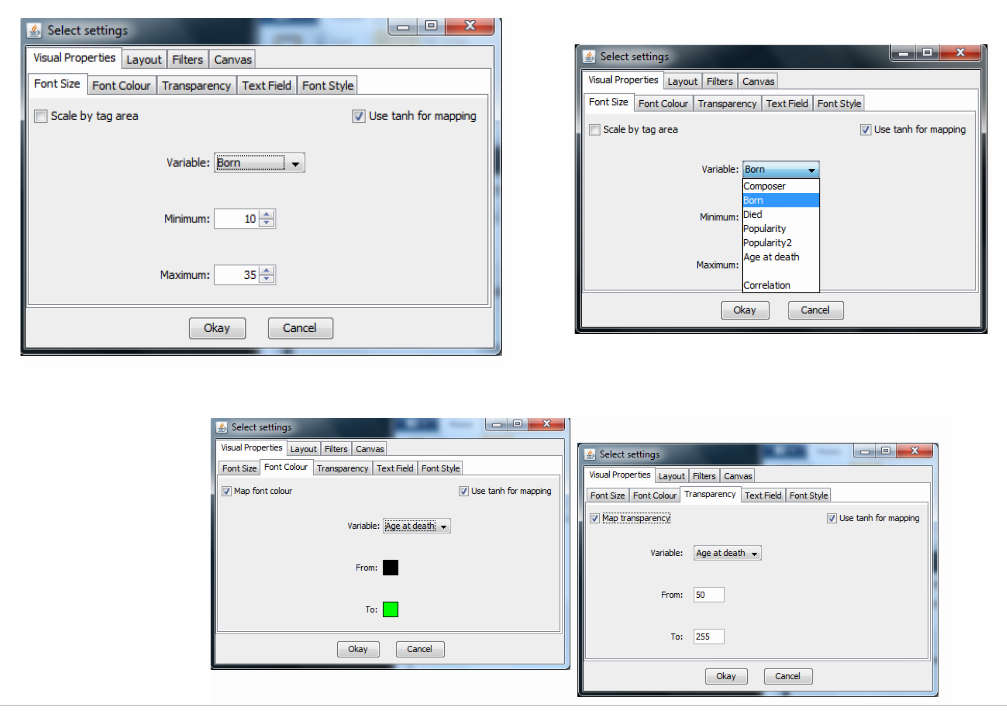
\includegraphics[scale=0.50]{interactivity-selectmapping.png}
	\caption{\emph{Interactivity}: Selection of mappings.}
	\label{fig:selectmapping}
\end{figure}

\begin{figure}[h!]
	\centering
	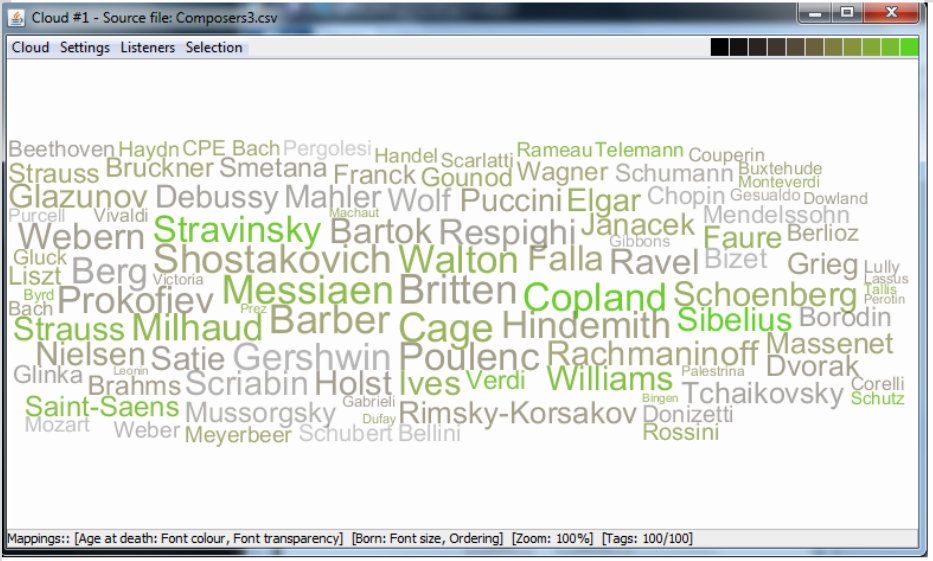
\includegraphics[scale=0.50]{interactivity-overview.png}
	\caption{\emph{Interactivity}: Overview.}
	\label{fig:overview}
\end{figure}

\begin{figure}[h!]
   \centering
   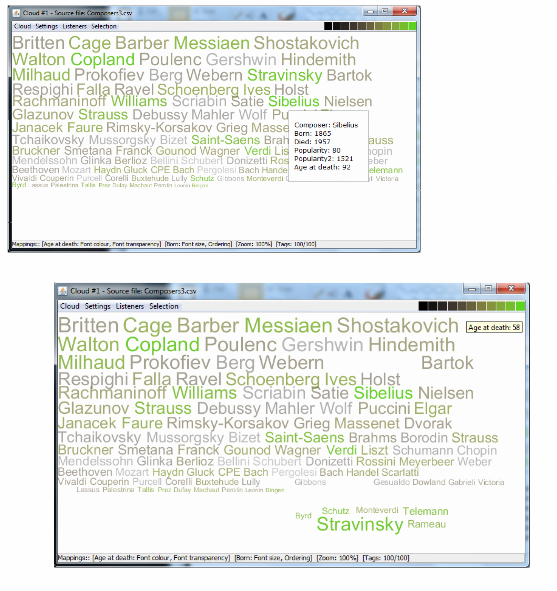
\includegraphics[scale=0.50]{interactivity-filter.png}
  \caption{\emph{Interactivity}: Filter and details-on-demand.}

	\label{fig:filter}
\end{figure}

% ------------------------------------------------------------------------

%%% Local Variables: 
%%% mode: latex
%%% TeX-master: "../thesis"
%%% End: 
